\documentclass[12pt]{article}
\usepackage{graphicx}
\usepackage[margin=1in]{geometry}
\usepackage{setspace}
\usepackage{booktabs}
\usepackage{hyperref}
\usepackage{float}
\usepackage{natbib}

\title{How does Height and Weight Affect NBA Player Performance}

\author{Justin Chan\\
	Jun Yan\\[2ex]
	Department of Statistics\\
	University of Connecticut\\
}

\begin{document}

\maketitle
\doublespace

\begin{abstract}

As basketball players get better and better at their craft in the modern age, players are doing everything 
they can to get an advantage over another. With practice, coaches, and trainers players can work hard at 
mastering their craft but what about the more physical aspects of their game? How does a players' height
and weight impact the performance ability of an NBA Player? Does being taller translate to scoring more
points per game? Does weight increase the amount of rebounds you will grab? Answers to such questions
will offer valuable insight to coaches, scouts, and analysts in making data-driven decisions for their teams.
This paper aims to determine whether, and to what extent, a player's height and weight influence their 
effectiveness in scoring, rebounding, assisting and other metrics through the use of linear regression and
machine learning techniques.

\bigskip
\noindent{\sc Keywords}:
Height and Weight;
Physical;
NBA;
Scoring Ability;
Rebounding Ability;
Assisting Ability;
Linear Regression;
Performance Metrics;
Sports Statistics

\end{abstract}

\section{Introduction}
\label{sec:intro}

Starting with the introduction, the paper will first go into the dataset being used and give a brief summary on the 
variables in the dataset and where the dataset has been collected located in Section~\ref{sec:data}. Following this
will be the Methods section, located in Section~\ref{sec:meth}. This is where the general methodology for the paper
will be explained. The Results section will be next which is where the findings of the research will be found a long 
with any relevant figures. This is located in Section~\ref{sec:resu}. Lastly, the paper will conclude with a Discussion 
section, in Section~\ref{sec:disc} that restates the aim, conclusions, and other important considerations of the paper.
As far as similar research, a study published in the British Journal of Sports Medicine looked at height as a predictor 
within all sports and found that height and sporting success was highly dependent on the type of sport \citep{tucker2012makes}. 
Another study done by head researcher Shaoliang Zhang looked at height and weight as a single predictor along with 
league experience \citep{zhang2017performance}. This paper would build onto that by looking at how player 
performance is affected by height and weight individually within the sport of basketball.

\section{Data}
\label{sec:data}

The dataset used for this analysis is take from Kaggle at \href{https://www.kaggle.com/datasets/justinas/nba-players-data}{NBA Players} 
which sourced its data from the NBA website and Basketball Reference. There are 12.8 thousand observations
with 22 variables taken from 1996 to 2022. It gives the per game averages of each player per season along with
other variables including height and weight. Specifically, the variables include age, games played, points per game,
rebounds per game, assists per game, and net rating. The data has been cleaned with no rows of missing data or
other data quality issues.

Before going into a deeper analysis, it was necessary to prepare the predictor variables to see if they were ready to
be fit within a linear regression model. To check the normality of both the height and weight variables, histograms
were produced:

\begin{figure}
	\caption{Predictor Variable Histograms}
	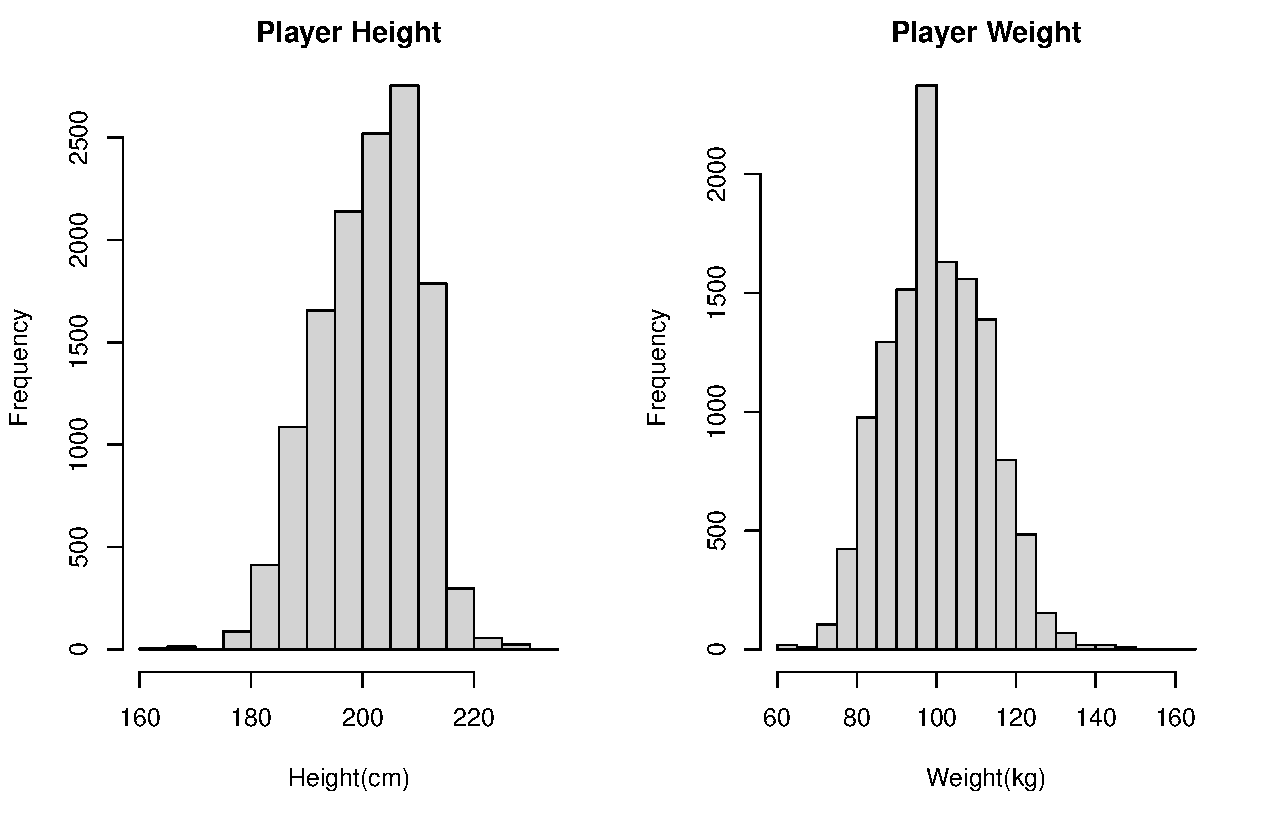
\includegraphics[width=1\textwidth]{predhistograms.pdf}
	\label{fig:predhistograms}
In Figure~\ref{fig:predhistograms}, the plots show the distribution of the predictors height and weight.
\end{figure}

As shown, the histograms produced seem to be relatively normal, meaning that we can proceed with further analysis
without having to worry about transforming our predictors in any way.

\section{Methods}
\label{sec:meth}

Since all of our predictors were seen to be following a normal distribution and all of our predictors seem ready to be fit
to model, to start, the data will be split into a training and testing dataset. Using a random sampling technique, there 
will be an 70\% to 30\% split allocated for training and testing, respectively with the seed set to 1 for reproducibility. 

The primary statistical tool used in this study was linear regression, a method chosen for its simplicity and interpretability. 
Multiple models were constructed to assess the impact of height and weight, both individually and collectively, on 
various performance metrics such as points scored (pts), rebounds (reb), assists (ast), and true shooting 
percentage (ts\_pct). Each of these metrics was treated as a dependent variable in separate regression models.

For each performance metric, three models were evaluated:

\begin{enumerate}
    \item A model considering both height and weight as predictors.
    \item A model considering only height as a predictor.
    \item A model considering only weight as a predictor.
\end{enumerate}

This approach allowed us to isolate the effect of each physical attribute on player performance. Furthermore, to 
ensure the validity of our models, we checked for multicollinearity, a common issue in regression analyses where 
predictors are highly correlated. The Variance Inflation Factor (VIF) was calculated for the model including both 
height and weight as predictors. A VIF of 3.13 indicated low correlation between height and weight, suggesting 
that multicollinearity would not significantly bias our results.

\section{Results}
\label{sec:resu}

The regression analysis conducted provided insight into the relationship between NBA players' physical attributes 
and their performance metrics. Our findings are summarized in the tables below, which present the R-squared 
and P-value for each of the models considered.

Table~\ref{tab:pts} presents the results for the points scored (pts) models. The R-squared values indicate that 
both height and weight, when considered together, account for a small portion of the variance in points scored (0.38\%). 
Individual analyses of height and weight yield even lower R-squared values, suggesting limited predictability of 
points scored by these variables alone. Notably, the P-values for these models are significantly low, indicating 
that the models are statistically significant despite the low explanatory power.

In Table~\ref{tab:reb} focusing on rebounds (reb), the model incorporating both height and weight demonstrates 
an R-squared value of 20.29\%, showing a more substantial relationship with the rebounding ability. The individual 
analyses of height and weight also reveal significant models, with height having a slightly lower R-squared value 
than weight.

Assists (ast), as shown in Table~\ref{tab:ast}, have a comparable explanatory power to rebounds when height and 
weight are considered together, with an R-squared of 19.95\%. The separate analyses for height and weight also 
reflect substantial explanatory power, albeit lower for weight alone.

Lastly, the true shooting percentage (ts\_pct) models presented in Table~\ref{tab:true} show a low variance explained 
among the performance metrics, with the highest R-squared value being 0.54\% for the combined height and weight 
model. However, the P-values indicate statistical significance in these models.

\begin{table}[ht]
\caption{Points}
\label{tab:pts}
\centering
\begin{tabular}{rrrr}
  \hline
 & HeightWeight & Height & Weight \\ 
  \hline
RSquared & 0.0038 & 0.0024 & 0.0004 \\ 
  PValue & 0.0000 & 0.0000 & 0.0721 \\ 
   \hline
\end{tabular}
\end{table}

\clearpage

\begin{table}[ht]
\caption{Rebounds}
\label{tab:reb}
\centering
\begin{tabular}{rrrr}
  \hline
 & HeightWeight & Height & Weight \\ 
  \hline
RSquared & 0.2029 & 0.1764 & 0.1922 \\ 
  PValue & 0.0000 & 0.0000 & 0.0000 \\ 
   \hline
\end{tabular}
\end{table}

\begin{table}[ht]
\caption{Assists}
\label{tab:ast}
\centering
\begin{tabular}{rrrr}
  \hline
 & HeightWeight & Height & Weight \\ 
  \hline
RSquared & 0.1995 & 0.1994 & 0.1404 \\ 
  PValue & 0.0000 & 0.0000 & 0.0000 \\ 
   \hline
\end{tabular}
\end{table}

\begin{table}[ht]
\caption{True Shooting Percentage}
\label{tab:ts}
\centering
\begin{tabular}{rrrr}
  \hline
 & HeightWeight & Height & Weight \\ 
  \hline
RSquared & 0.0054 & 0.0054 & 0.0039 \\ 
  PValue & 0.0003 & 0.0000 & 0.0000 \\ 
   \hline
\end{tabular}
\end{table}



\section{Discussion}
\label{sec:disc}

Still in progress

\bibliography{references}
\bibliographystyle{plainnat}
\end{document}
	